\documentclass[12pt]{article}
\author{GUILBERT Augustin, MARTINANT Valentin, OZDEMIR Serdar} 
\date{\today}
\title{\textsc{\textbf{Compression d'images}}}
\renewcommand{\baselinestretch}{1.2}
\usepackage{graphicx}
\usepackage[utf8]{inputenc} %accent
\usepackage[T1]{fontenc} %accent
\usepackage[frenchb]{babel} % choix de la langue 
\usepackage{graphicx} %inclure des images(PNG,JPG,PDF)
\usepackage{amsmath,amssymb}
\usepackage[top=2.5cm,bottom=2.5cm,left=2.5cm,right=2.5cm]{geometry}
\usepackage{fancyhdr}
\usepackage{caption}
\pagestyle{fancy} 
\lfoot{TIPE Compression d'images} 
\rfoot{Lycée Blaise Pascal 2016-2017} 

\renewcommand{\footrulewidth}{0.8pt}

\begin{document}
\maketitle
\newpage
\tableofcontents
\newpage
\section{Objectifs et types de compression d'images}	
Les images peuvent être codées « naïvement » : il s’agit d’enregistrer une matrice contenant pour chaque pixel: la valeur de celui-ci s’il s’agit d’une image en noir et blanc, les valeurs rouge, verte et bleues si c’est une image en couleur. Ce format est simple à mettre en œuvre et facile à décoder, cependant il est très gourmand en stockage.  Par exemple pour image couleur de taille 500*500 (taille moyenne), il faut près de 75000 octets soit 600000bits ! Ce qui peut s’avérer problématique pour le stockage de grandes quantités d’images, mais aussi lors des transferts. C’est pourquoi il est intéressant de compresser les images, c’est-à-dire diminuer leur poids. Deux types de compression se présentent à l’utilisateur.
D’une part, la compression sans perte, qui permet de conserver une netteté des traits irréprochable. Cette compression est utilisée pour des images nécessitant une très grande précision, tel que les schémas, les dessins techniques ou les balayages médicaux.
D’autre part, la compression avec perte privilégie par définition l’économie de poids à la qualité. Ce qui est utile dans le cas de transmission bas débit, ou pour un stockage de masse d’images, cependant la qualité de l’image est dégradée. Le format JPEG (Joint Photographic Expert Group) s’avère être un bon compromis entre une qualité d’image très correcte et une bonne compression. La compression JPEG s’appuie sur la DCT (Discrete Cosine Transform).
Nous avons réalisé à l’aide du logiciel de programmation Python une compression de type JPEG.


\newpage
\section{Compression JPEG}
La compression JPEG permet une bonne qualité car elle utilise la DCT. En effet, la DCT permet de traduire l'information spatiale des pixels en une information fréquentielle. Or, les variations rapides d’intensités, traduites pas les hautes fréquences étant rares, et l’œil humain les percevant mal, elles sont supprimées au cours de la compression. Une image à laquelle on applique la compression JPEG suit le traitement suivant.
\paragraph{}
\begin{center}
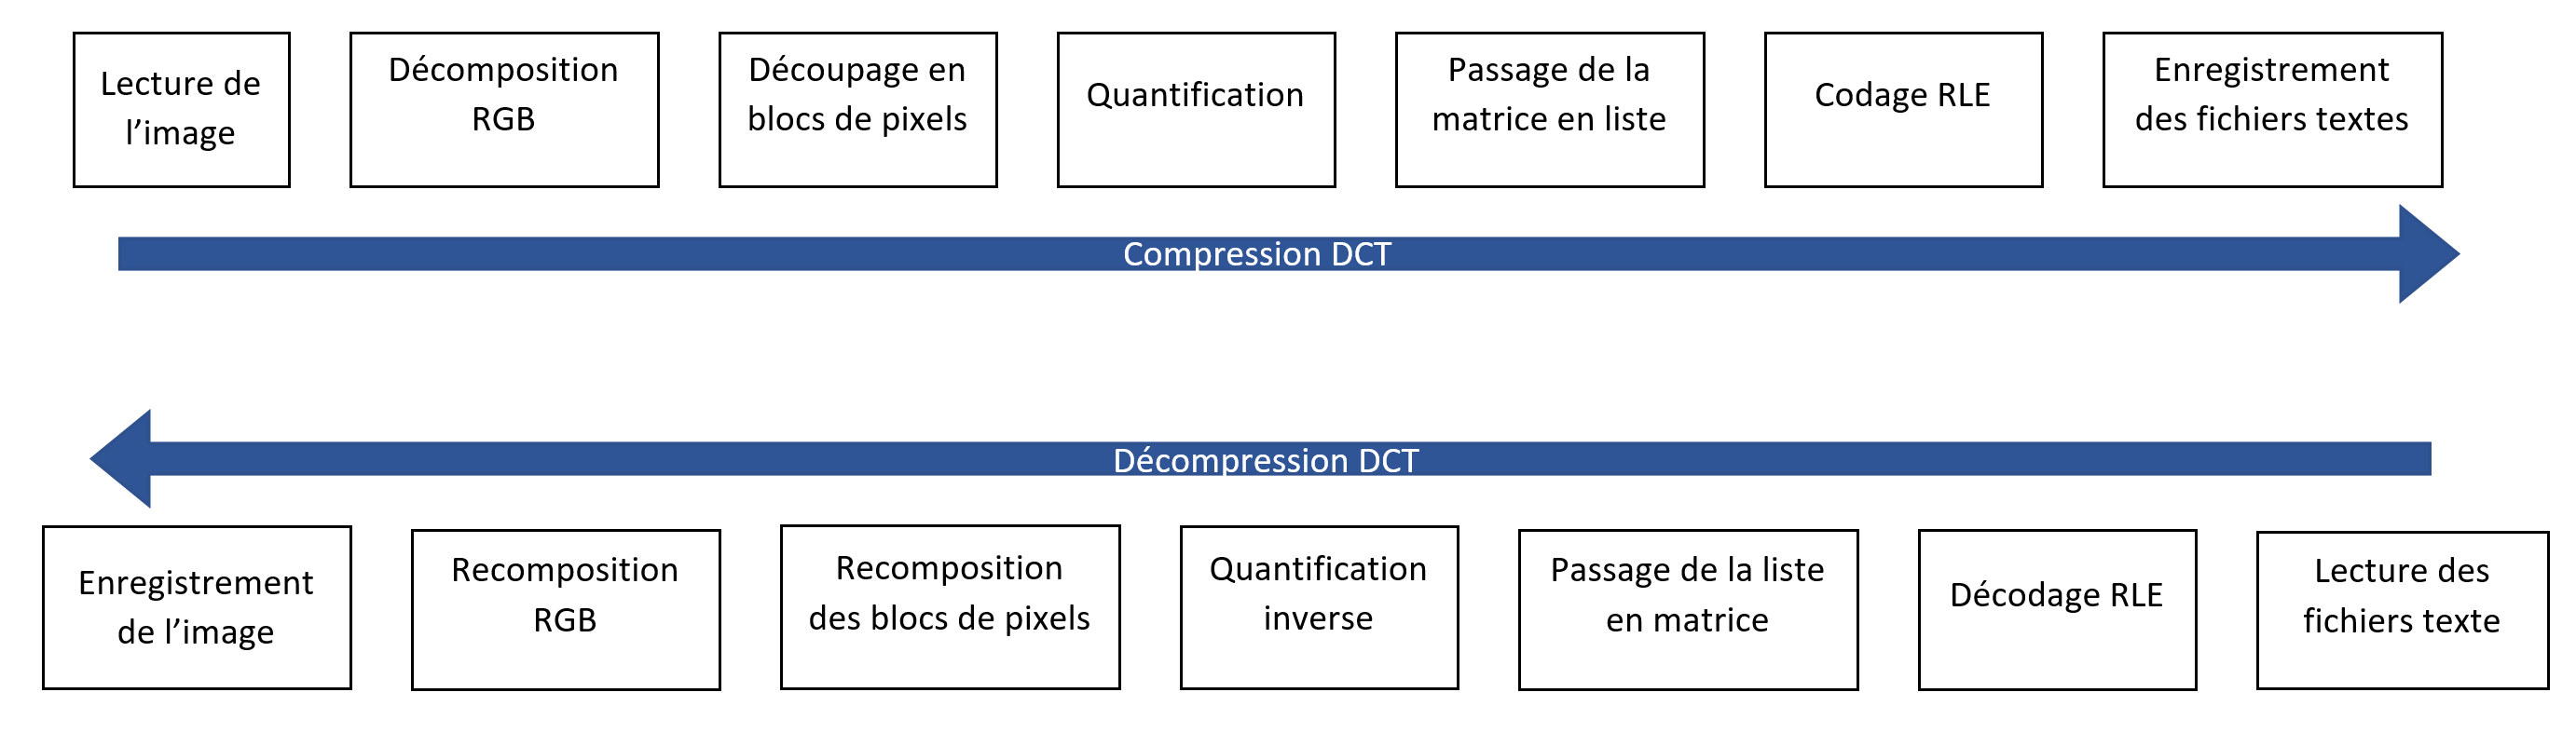
\includegraphics[scale=0.2]{schema_dct_new.png} %scale pour augmenter ou diminuer proportionnellement la hauteur et largeur de l'image
\end{center}
\paragraph{}
La formule de la Transformée en Cosinus Discrète (DCT) se définit de la manière suivante: 

\begin{equation*} 
C(i)(j)=\cfrac{1}{\sqrt{2N}} \biggl[\sum_{1\leq x\leq N-1} \sum_{1\leq y\leq N-1} p(x,y) \cos{\biggl[\cfrac{(2x+1) i \Pi}{2N}}\biggr] \cos{\biggl[\cfrac{(2y+1) j \Pi}{2N}}\biggr]\biggr]
\end{equation*}

La première étape est la lecture de l’image qui consiste à la convertir en une matrice de dimension 3 (longueur, largeur, nombre de couleurs). Cette étape est suivie dans le cas d’une image en couleur par la décomposition de cette matrice en trois matrices contenant chacune les valeurs des pixels pour une couleur donnée. Il faut ensuite découper cette matrice en blocs carrés , pour des raisons de complexité de calcul on se limitera à une taille de 8, bon compromis entre temps de calcul et précision. Cette opération peut nécessiter le rajout de lignes et de colonnes si le nombre de lignes et de colonnes n’est pas un multiple de 8, les colonnes et lignes rajoutées sont alors des copies de la dernière ligne ou colonne propre à l’image, ainsi elles n’interfèrent pas dans la DCT. Ces blocs de matrices subissent alors un changement de base, permettant de faire apparaître les variations sous forme de fréquences. Mais cela reste encore une opération très couteuse: il faudrait parcourir chaque matrice et calculer une somme double pour chaque coefficient.
\paragraph{}

\paragraph{}
Pour éviter cela, on peut concevoir cette formule comme un changement de base avec la matrice de passage définie de la manière suivante:
\begin{center}
$P(i)(j)=
\begin{Bmatrix}
\cfrac{1}{\sqrt{2N}}  \qquad if \quad i=0 \\
\sqrt{\cfrac{2}{N}} \: cos\biggl[\cfrac{2*j+1}{2N}\biggr] \qquad if \quad i>0 \\
\end{Bmatrix}
$
\end{center}
\paragraph{}
Ce qui nous donne, une fois calculée numériquement:
\begin{center}

$P=
\begin{Bmatrix}

.3536& .3536& .3536& .3536& .3536& .3536& .3536& .3536 \\
.4904& .4157& .2778& .0975& -.0975& -.2778& -.4157& -.4904 \\
.4619& .1913& -.1913& -.4619& -.4619& -.1913& .1913& .4619 \\
.4157& -.0975& -.4904& -.2778 & .2778& .4904& .0975& -.4157 \\
.3536& -.3536& -.3536& .3536& .3536& -.3536& -.3536& .3536 \\
.2778& -.4904& .0975& .4157& -.4157& -.0975& .4904& -.2778 \\
.1913& -.4619& .4619& -.1913& -.1913& .4619& -.4619& .1913 \\
.0975& -.2778& .4157& -.4904& .4904& -.4157& .2778& -.0975 \\

\end{Bmatrix}
$
\end{center}

\paragraph{}
On réalise alors le changement de base suivant la formule suivante: P.M.P\up{-1} , la matrice de passage n'étant calculée qu'une fois, on réduit la complexité de O(n\up{4}) à celle des fonctions numpy.dot() utilisées dans notre programme pour multiplier plus efficacement 
\newline
\paragraph{}
 Arrive alors l’étape de la quantification qui consiste à diviser les coefficients de l’image par ceux d’une matrice de quantification: on ne conserve que les coefficients les plus importants : l'arrondi à la partie entière permet d'en réduire une bonne partie à 0. Nous avons retenu celle ci à un niveau de quantification de 10%
 \begin{center}
 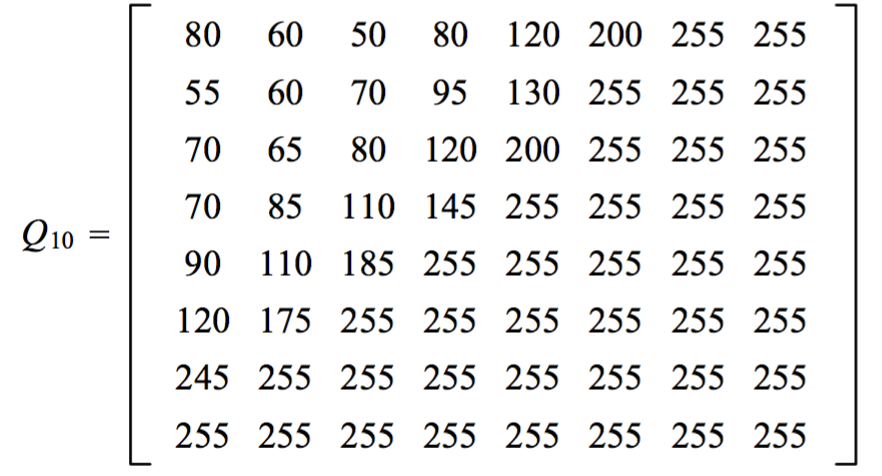
\includegraphics[scale=0.75]{photo1}
 \end{center}
\newpage
La Matrice obtenue après quantification est ensuite parcourue puis ses éléments ajoutés à une liste selon le schéma suivant :

 \begin{center}
 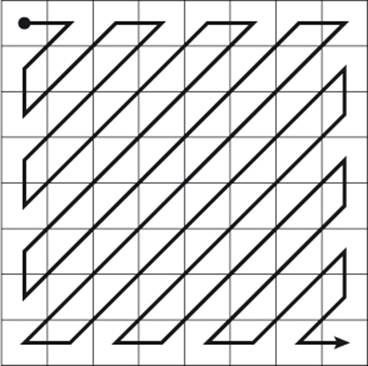
\includegraphics[scale=0.7]{image4}
 \end{center}
	
Cette liste contenant beaucoup de 0 consécutifs, elle subit une RLE (Run-Lenth Encoding), qui consiste à indiquer le nombre de coefficients de même valeur consécutifs et la valeur de ce coefficient. Enfin, ces listes sont enregistrées en tant que fichiers textes qui représentent l’image une fois compressée.
\newline
La décompression suit le chemin inverse: 
\newline
Tout d’abord, une fonction lit et transforme en liste les fichiers textes contenant l’image compressée, puis ces listes subissent une RLE inverse permettant d’obtenir 64 coefficients. 
On transforme ensuite cette liste en une matrice 8*8 selon le schéma diagonal défini plus haut dans le sens inverse. Les coefficients de la matrice sont ensuite multipliés par ceux de la matrice de quantification, puis on réalise le changement de base inverse. Les blocs de 64 pixels sont alors rassemblés, puis les colonnes et lignes rajoutées sont supprimées afin de donner à la matrice les dimensions de l’image d’origine. 
\newline
Finalement, les matrices des différentes couleurs sont assemblées puis cette matrice finale est enregistrée au format image pour donner une image finale de même taille que l’originale.
\newpage

\section{Résultats obtenus}
Lors de la compression, plus le niveau de quantification de l'image est faible, plus l’image est compressée, est donc la qualité dégradée. Nous avons testé différents niveaux de quantification sur une image afin de déterminer leur impact sur la compression.
\captionsetup{labelformat=empty}
\begin{table}[h]
\begin{center}
\begin{tabular}{|p{2,5cm}|p{3cm}|p{3,3cm}|p{2,5cm}|}
\hline
\centering Niveau de quantification&\centering Taille originale (en Mo)&\centering Taille compressée (en Mo)&\centering Taux de compression\tabularnewline%\centering permet de centrer le contenue de la cellule suiante, il faut alors utiliser \tabularnawline pour sauter la ligne car \\ est désactivé
\hline
\centering 10&\centering 6,22&\centering 1,08&\centering 5,7\tabularnewline
\hline
\centering 20&\centering 6,22&\centering 1,26&\centering 4,9\tabularnewline
\hline
\centering 30&\centering 6,22&\centering 1,44&\centering 4,3\tabularnewline
\hline
\centering 40&\centering 6,22&\centering 1,60&\centering 3,9\tabularnewline
\hline
\centering 50&\centering 6,22&\centering 1,76&\centering 3,5\tabularnewline
\hline
\centering 60&\centering 6,22&\centering 1,90&\centering 3,3\tabularnewline
\hline
\centering 70&\centering 6,22&\centering 2,14&\centering 2,9\tabularnewline
\hline
\centering 80&\centering 6,22&\centering 2,56&\centering 2,4\tabularnewline
\hline
\centering 90&\centering 6,22&\centering 3,39&\centering 1,8\tabularnewline
\hline

\end{tabular}
\end{center}
\caption{Taux de compression en fonction du niveau de quantification choisi}
\end{table}
\newpage
Ainsi, la compression de l’image reste imperceptible pour un niveau de quantification supérieur à 50, en effet, un niveau de quantification trop faible entraine l’uniformisation des pixels de chaque carré de 64 pixels, ce qui dégrade amplement la qualité de l’image. Voici les images obtenus pour des niveaux de compression de 90, 50, et 10.
\newline
\begin{figure}[h]
    \begin{minipage}[c]{.46\linewidth}
        \centering
        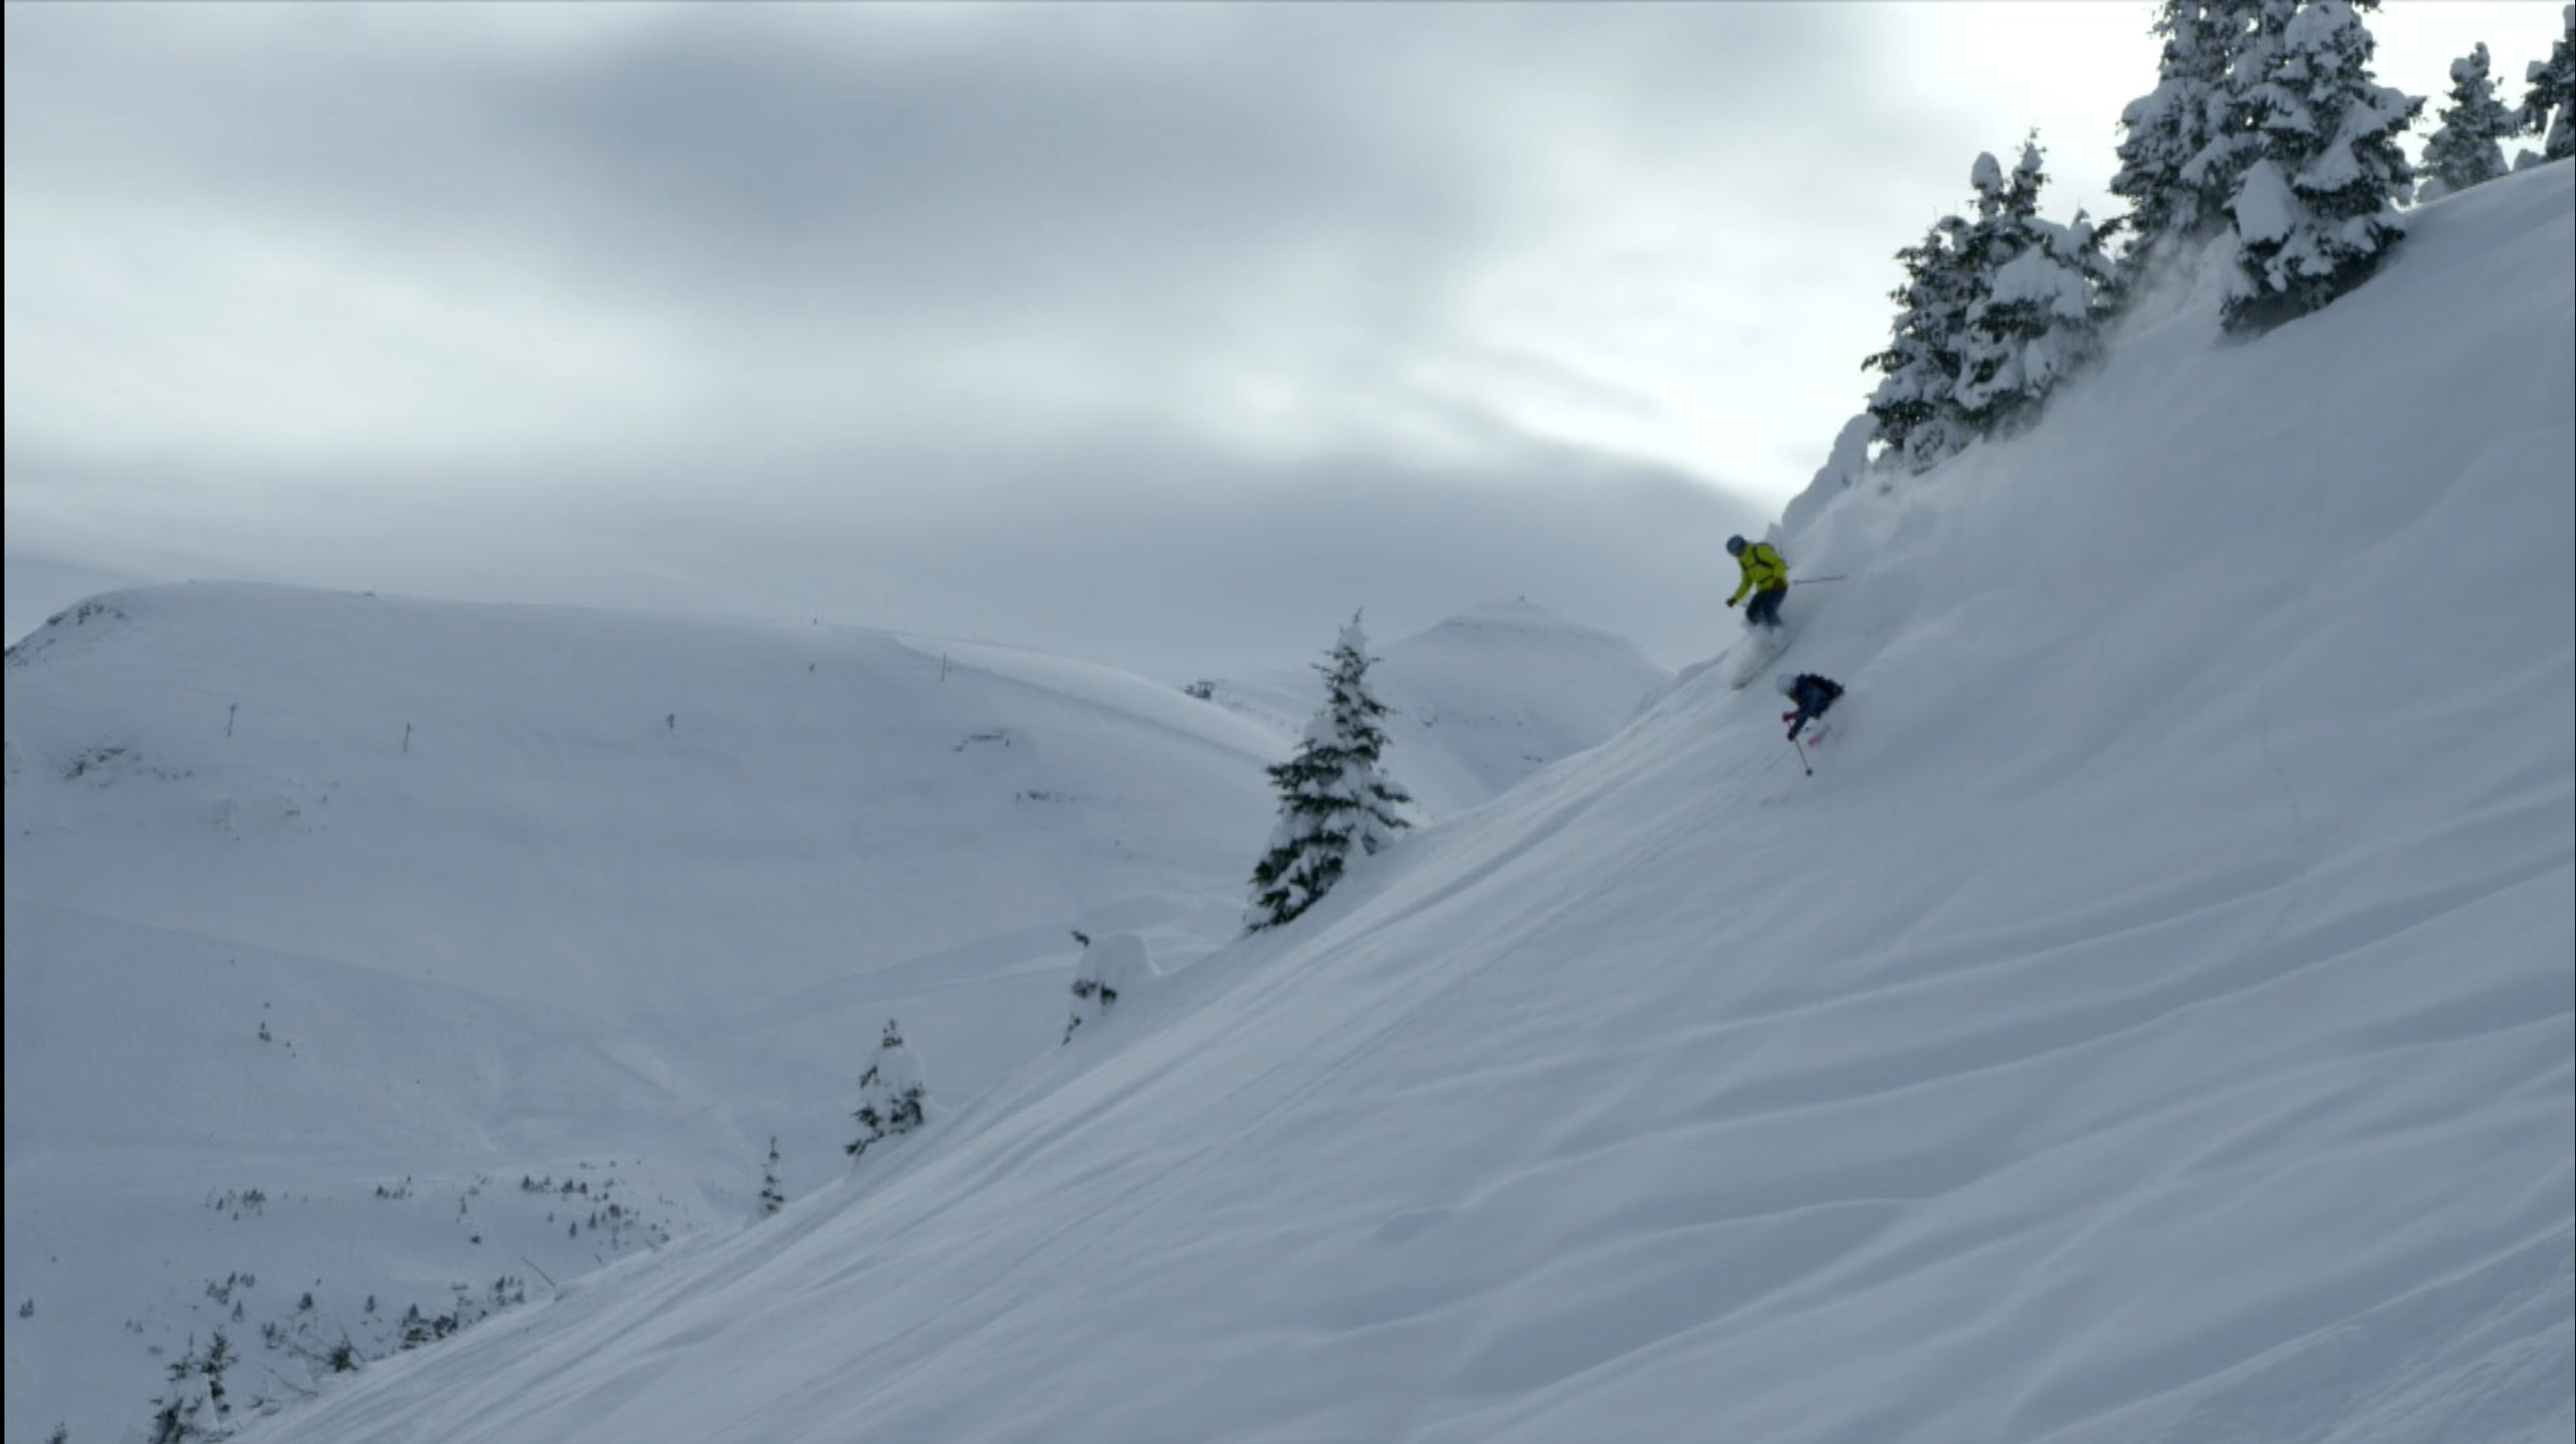
\includegraphics[scale=0.1]{skilatex}
        \caption{Image originale}
    \end{minipage}
    \hfill%
    \begin{minipage}[c]{.46\linewidth}
        \centering
        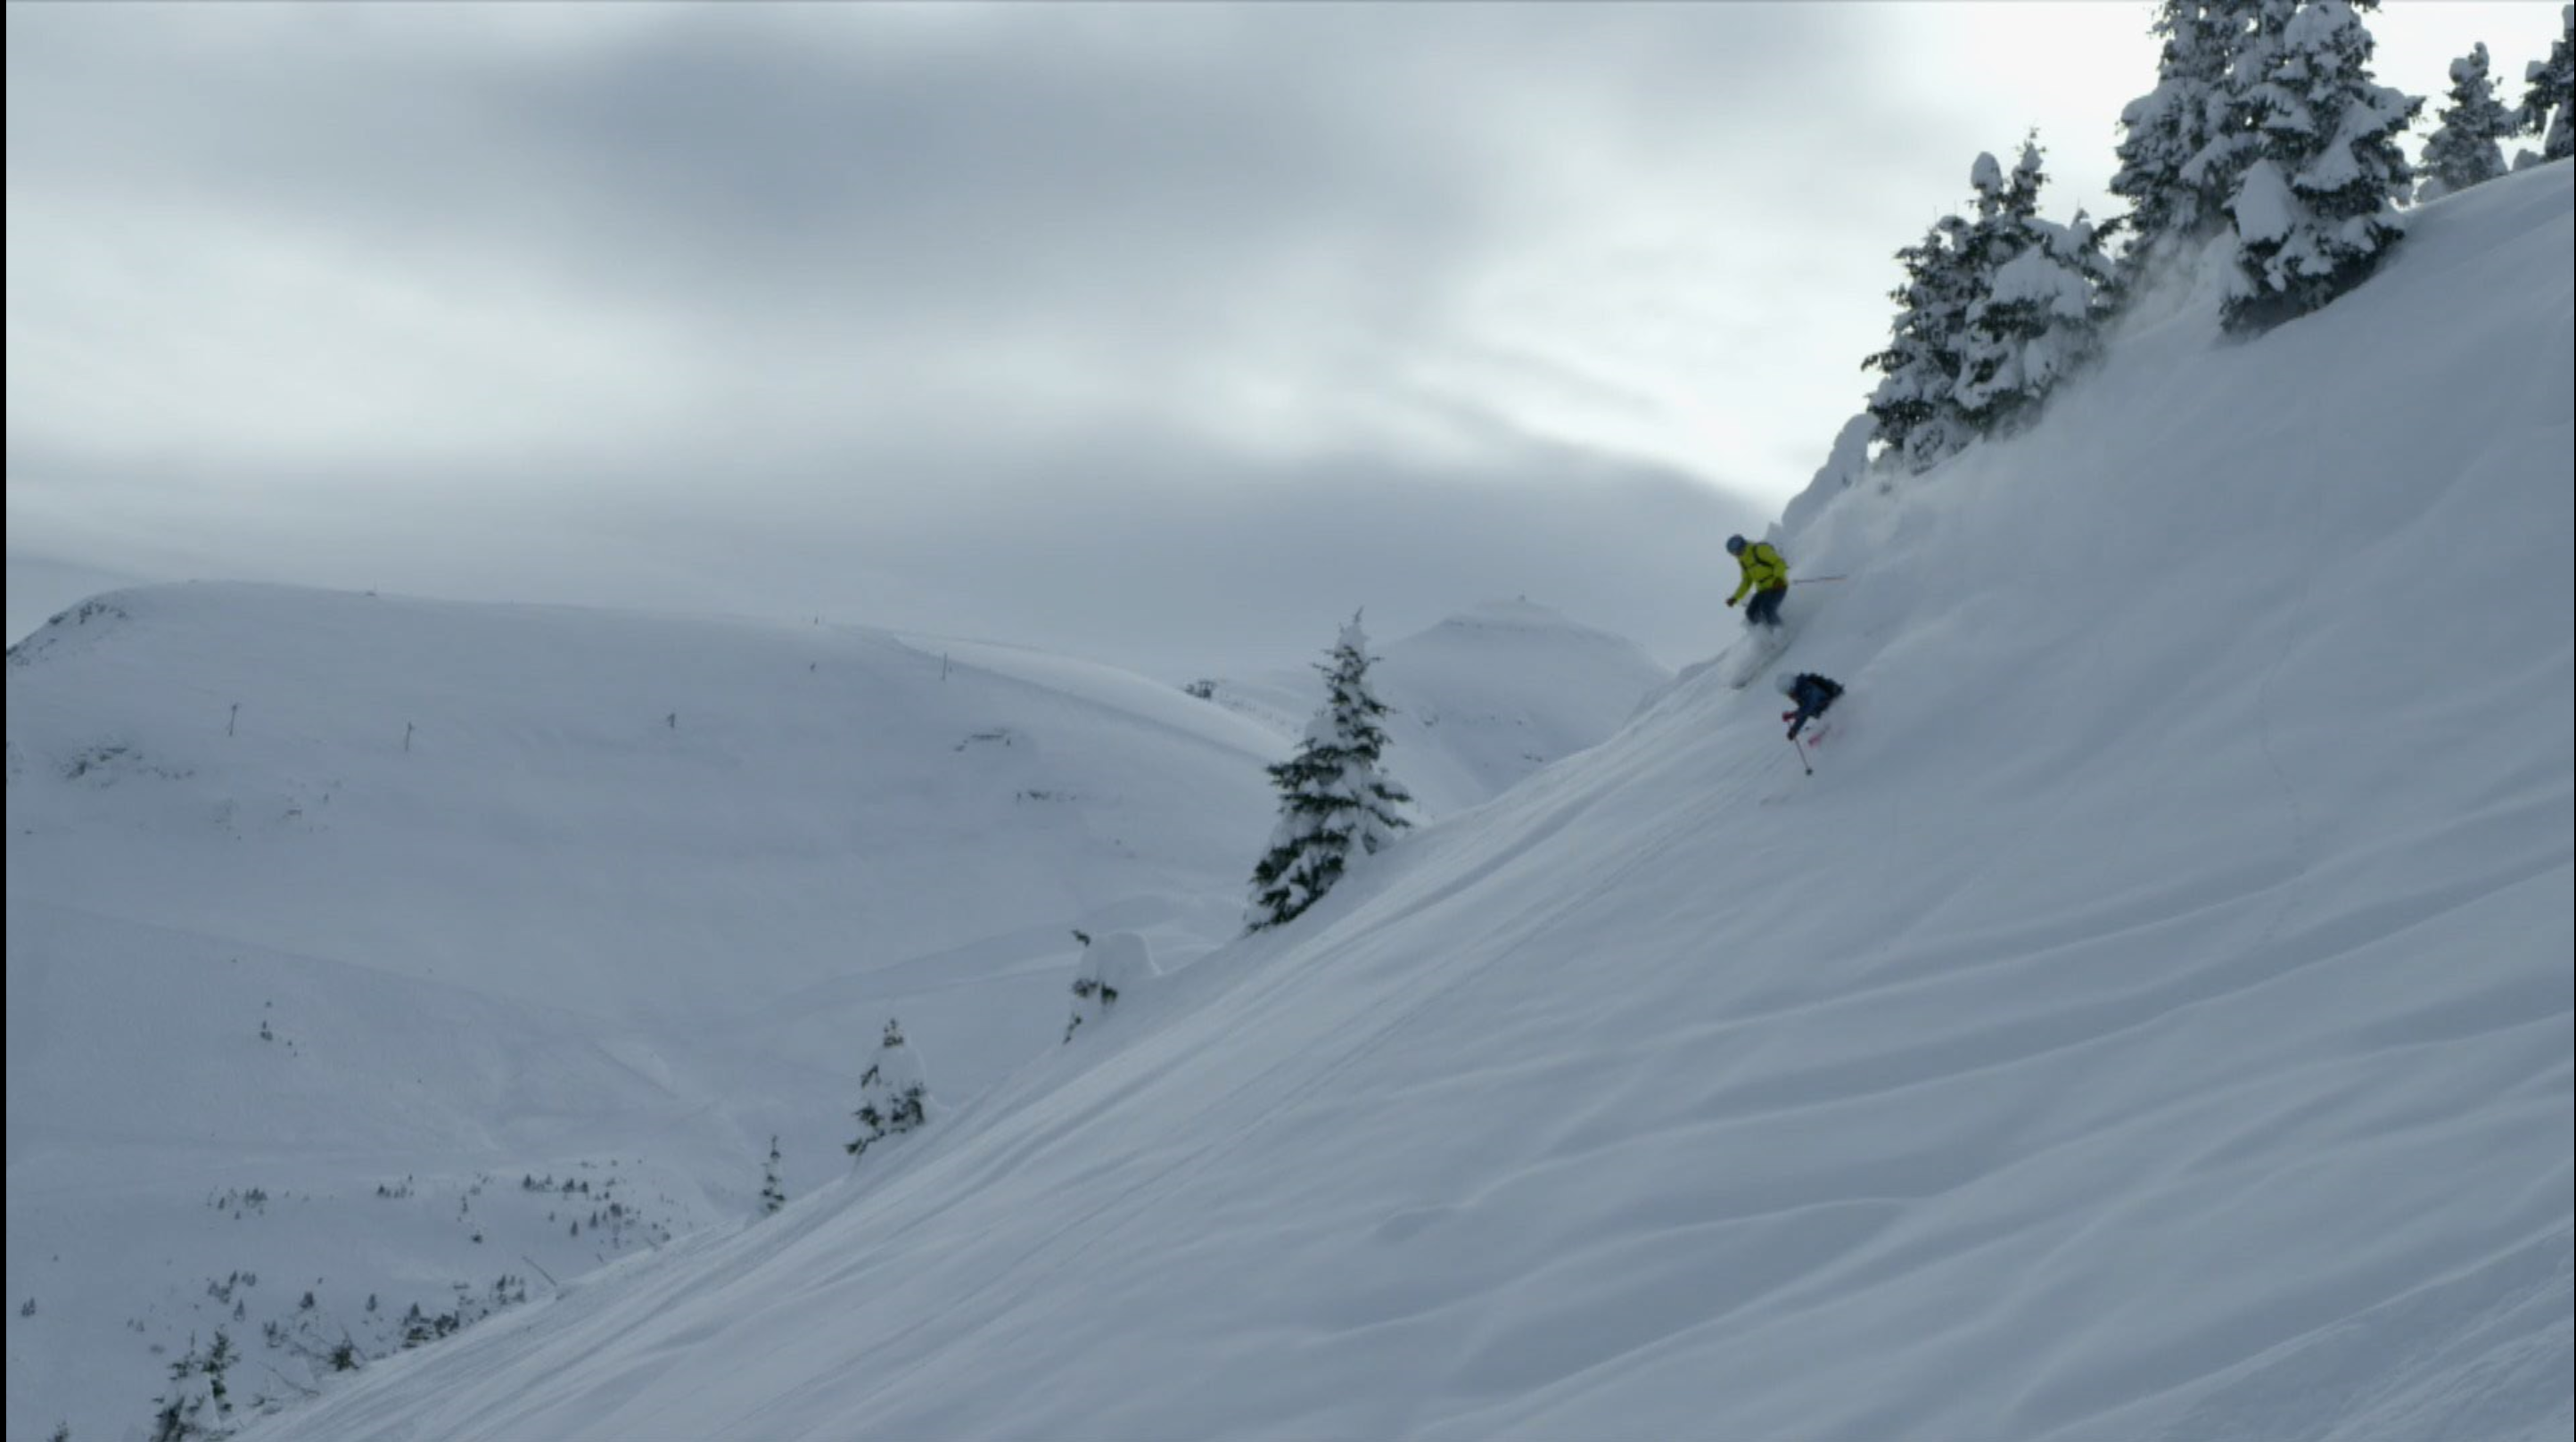
\includegraphics[scale=0.1]{skilatex90}
        \caption{Niveau de compression de 90}
    \end{minipage}
\end{figure}
\begin{figure}[h]
    \begin{minipage}[c]{.46\linewidth}
        \centering
        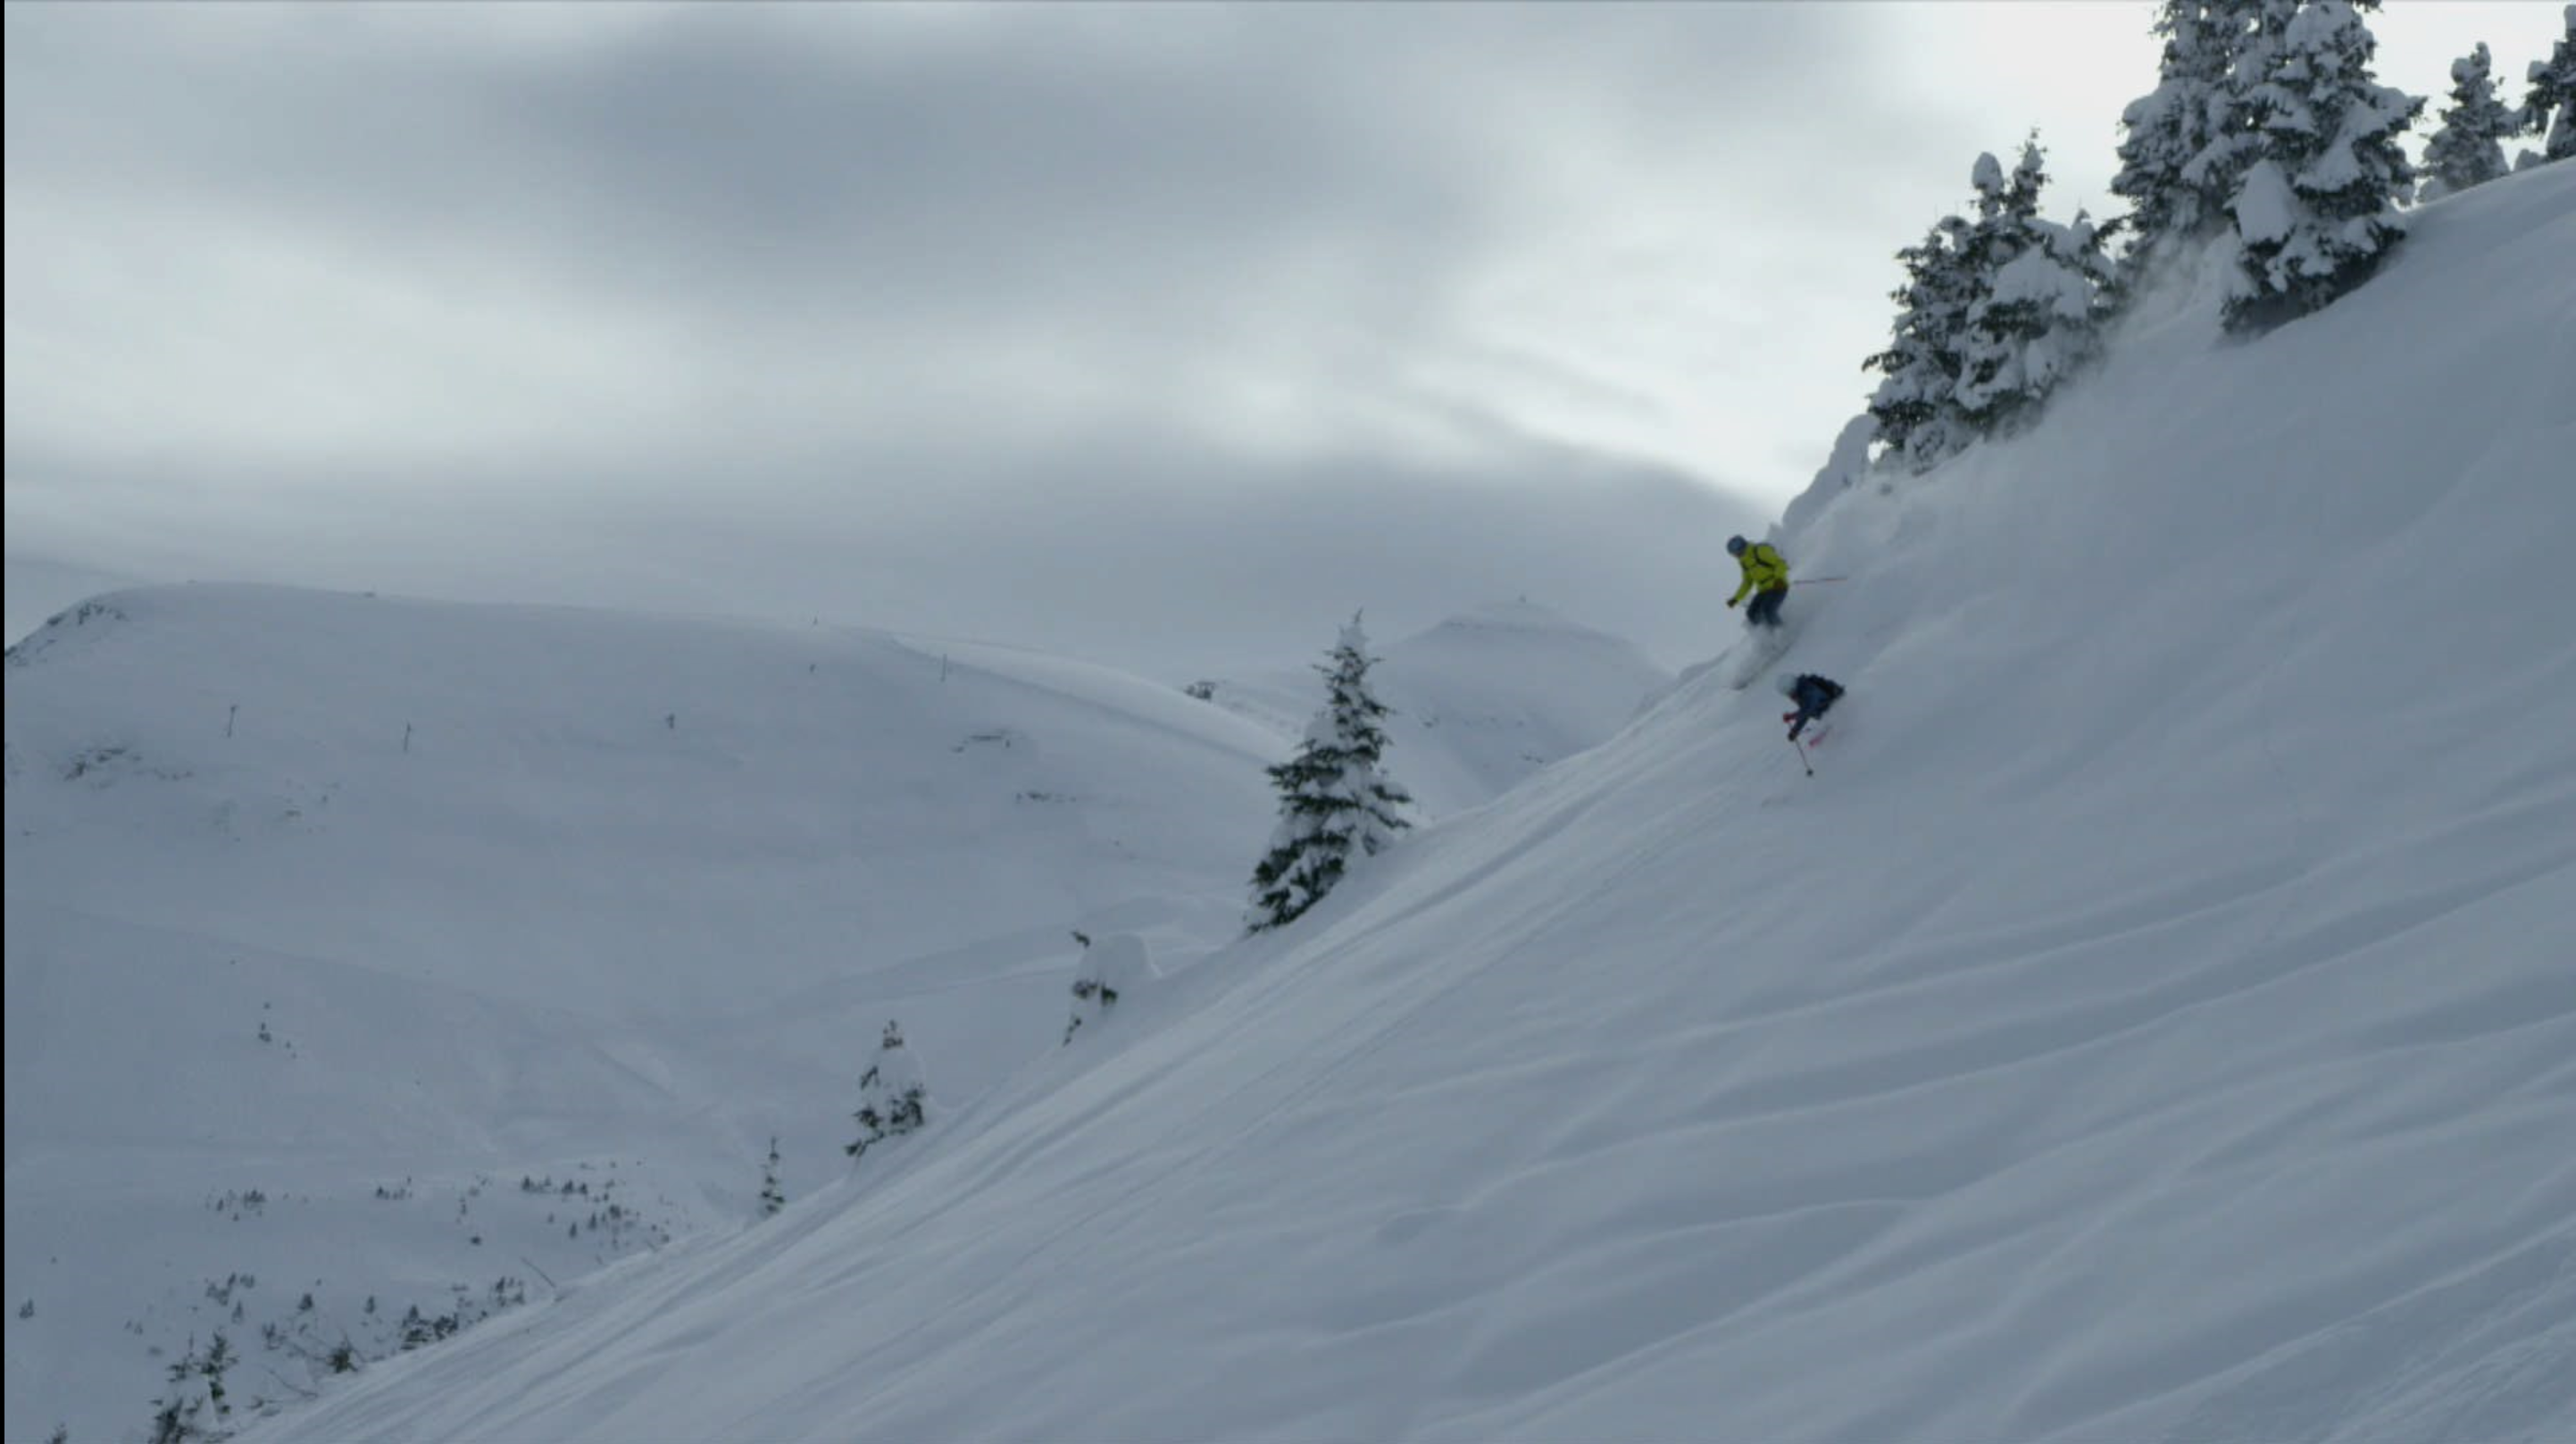
\includegraphics[scale=0.1]{skilatex50}
        \caption{Niveau de compression de 50}
    \end{minipage}
    \hfill%
    \begin{minipage}[c]{.46\linewidth}
        \centering
        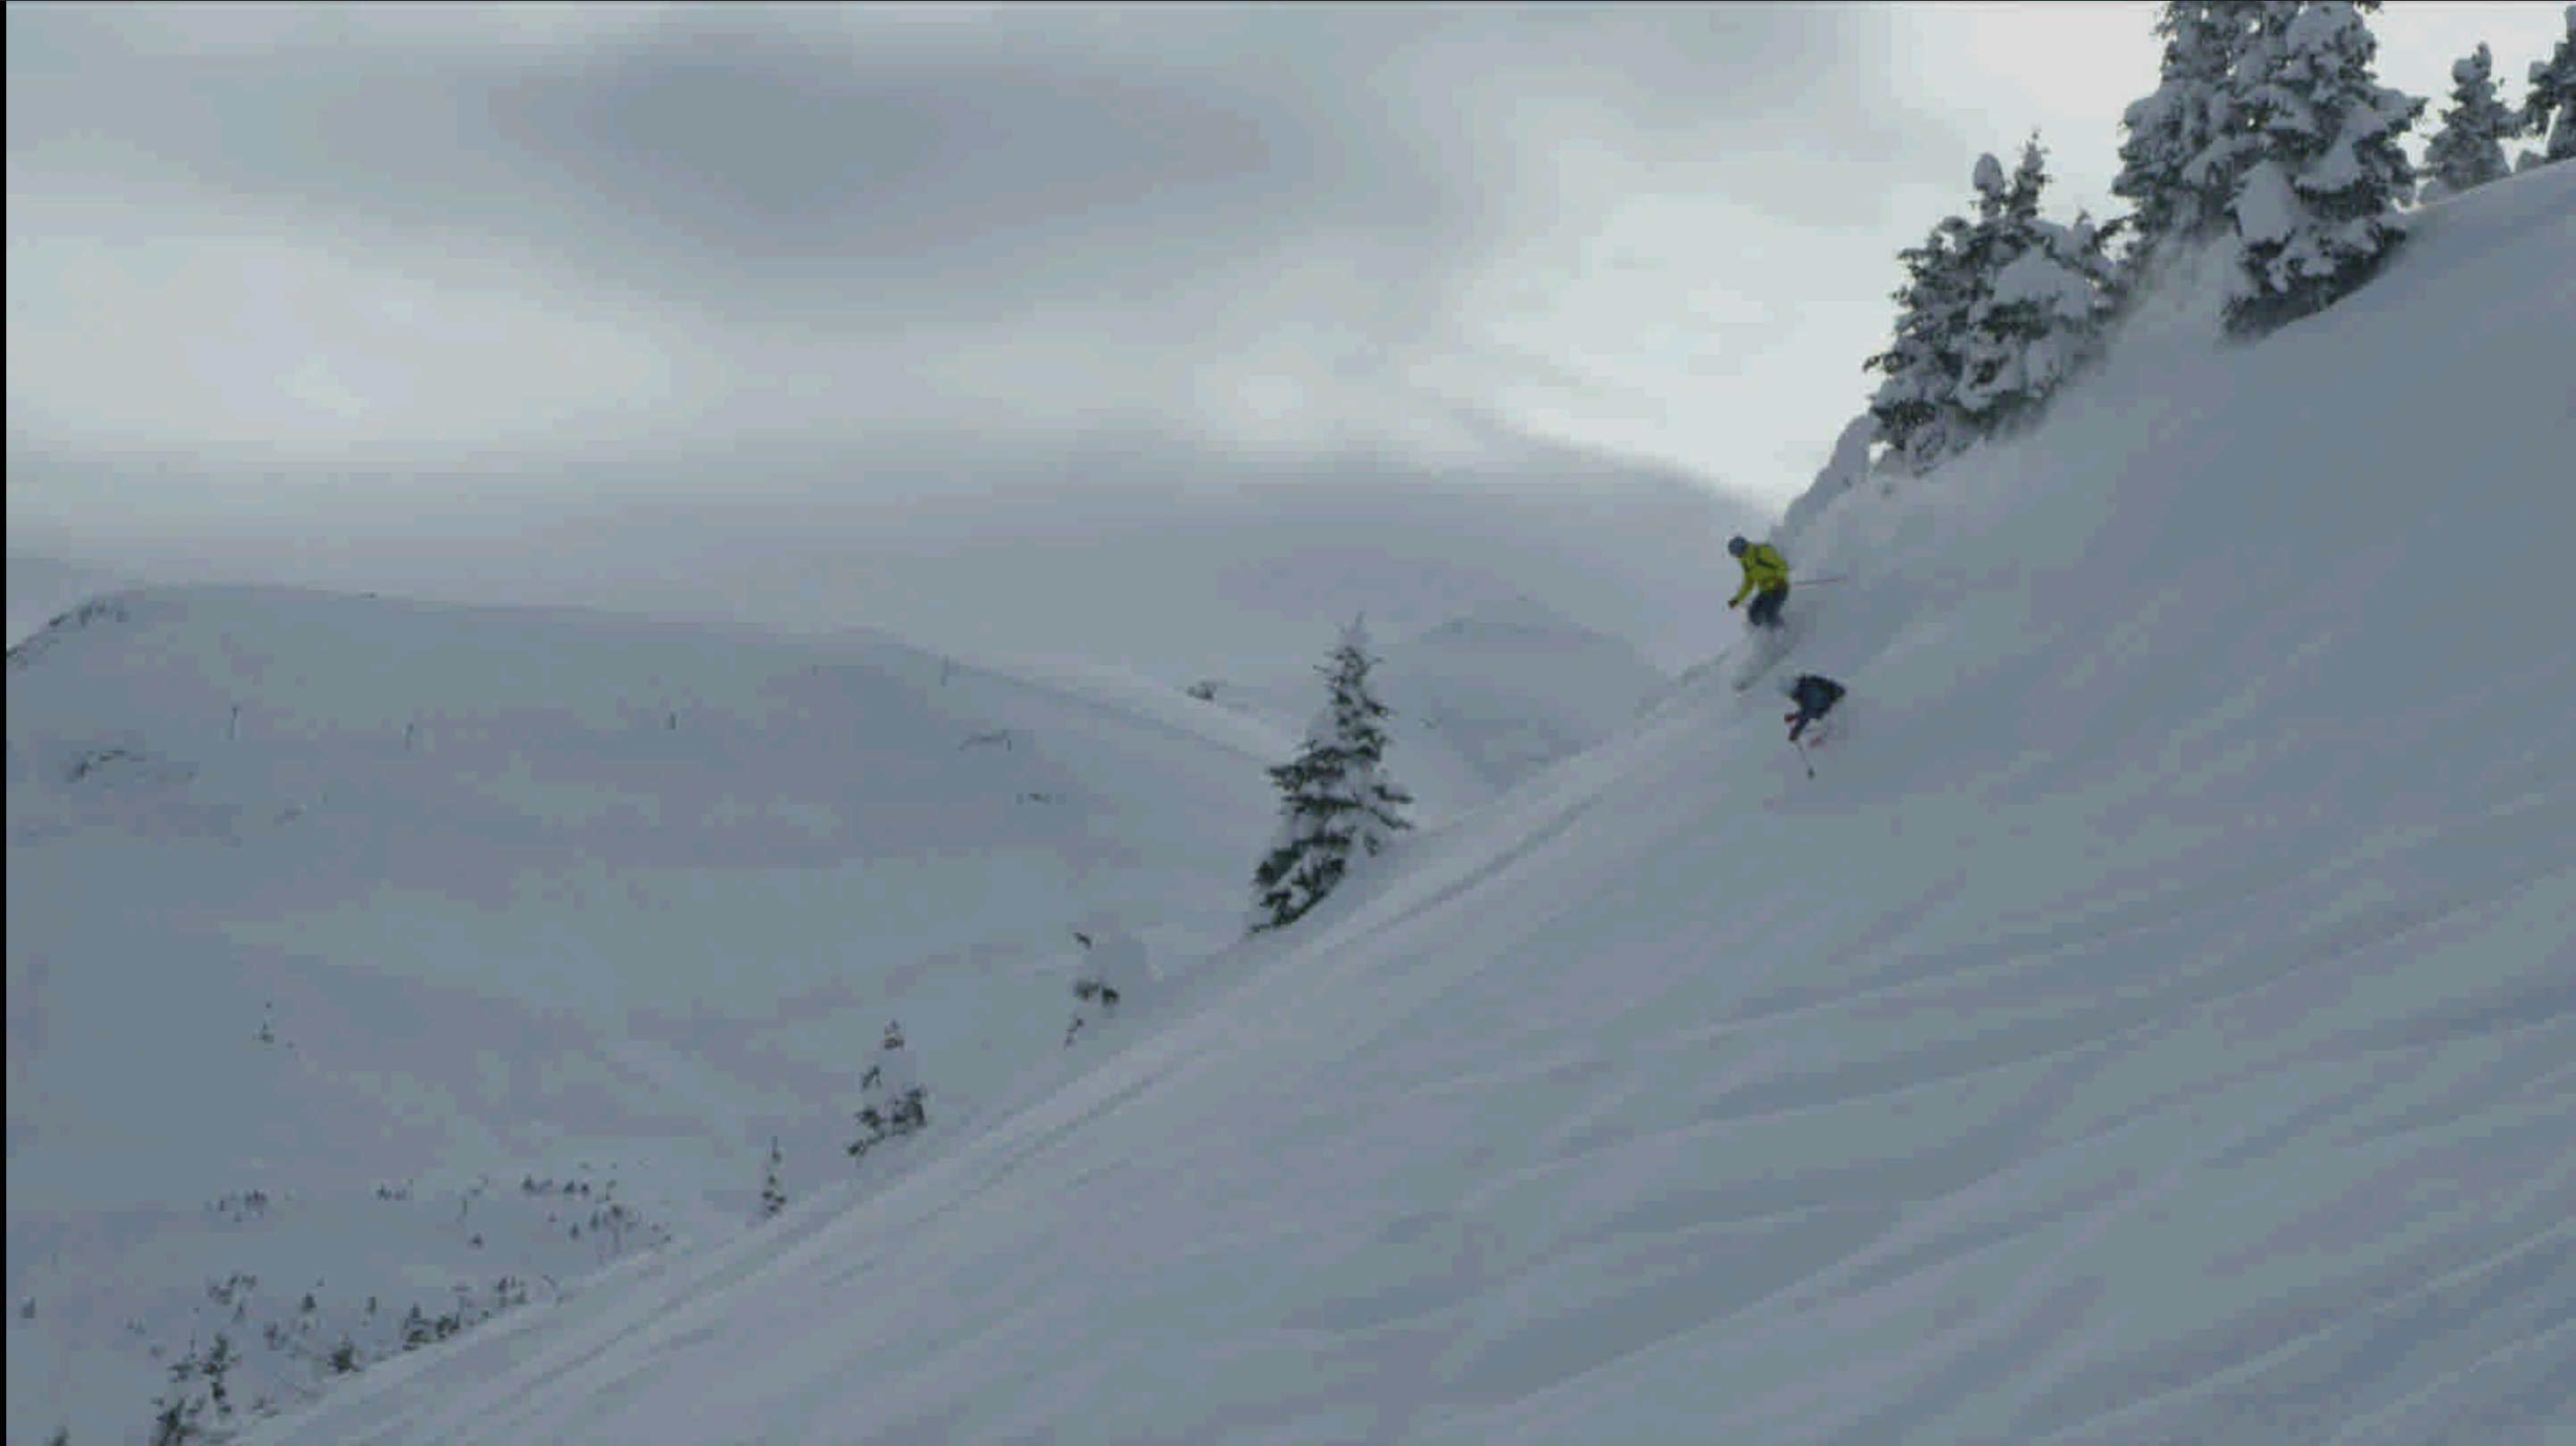
\includegraphics[scale=0.1]{skilatex10}
        \caption{Niveau de compression de 10}
    \end{minipage}
\end{figure}
\paragraph{}
Les compressions avec pertes officielles peuvent avoir des taux de compressions allant de 3 à 100, ce qui est beaucoup plus important que ce que nous réalisons, car nous obtenons un taux maximal de 9 pour des images de très mauvaise qualité. En effet, notre programme n'est pas optimal pour plusieurs raisons: les fichiers textes de la compression sont codés en tant que caractères qui plus est avec des caractères séparateurs et non pas en hexadécimal, privilégié normalement, ce qui permettrait un gain de place, le temps de compression est élevé.
\newpage
\section{Bibliographie}
\paragraph{}
$http://lmrs.univ-rouen.fr/Vulgarisation/JPEG/jpeg-DCT.html$
\paragraph{}
$http://etud.insa-toulouse.fr/~flone_sa/BEmultimedia/index.php?Dct$
\paragraph{}
$http://igm.univ-mlv.fr/~dr/XPOSE2013/La_compression_de_donnees/jpeg.html$
\paragraph{}
$http://www-ljk.imag.fr/membres/Valerie.Perrier/SiteWeb/node9.html$
\paragraph{}
$https://www.math.cuhk.edu.hk/~lmlui/dct.pdf$
\newline
\underline{Image compression and the discrete cosine transform}, Ken Cabeen and Peter Gent

\newpage
\section{Abstract}
Currently, everybody stores a lot of pictures on numerous devices, like computers or smartphones. Nevertheless, people needs to store more and more pictures, so pictures must be compressed. A compressed picture is lighter than a non-compressed one, but quality is damaging during this process. JPEG format is one of the best because it combines a good compression rate and a good quality. JPEG compression principle is based on DCT which transform pixels information into frequencies. High frequencies mean fast intensity changes, well fast intensity changes are occasional in pictures, and human eyes don’t detect it. So, these frequencies are deleted during the compress to create a lighter picture.

\end{document}
